\chapter{Variational formulation} \label{chapter:variational_fft}

In following chapter a detailed overview of the variational FFT-based homogenization procedure proposed by \cite{vondrejc_fft-based_2014}, \cite{zeman_finite_2017} and \cite{de_geus_finite_2017} is presented.
It follows closely the descriptrions found in \cite{zeman_finite_2017} in what concerns small strains and \cite{de_geus_finite_2017} regarding large strains.
The small strain case is introduced first and then the necessary changes to extend it to large strains are described.


\section{Local problem and its weak form}

In what follows, the microstructure of the material is to be represented by a periodic cell \(\Omega_\mu\). In two dimensions, \(\Omega_\mu=\left(-l_{1} / 2, l_{1} / 2\right) \times\left(-l_{2} / 2, l_{2} / 2\right)\)\nomenclature[V]{$\Omega_\mu$}{RVE domain} with area \(v_{\mu,0}=l_{1} l_{2}\).
In three dimensions, \(\Omega_\mu=\left(-l_{1} / 2, l_{1} / 2\right) \times\left(-l_{2} / 2, l_{2} / 2\right)\times\left(-l_{3} / 2, l_{3} / 2\right)\) with volume \(v_{\mu,0}=l_{1} l_{2} l_{3}\).
The material response at a point \(\bm Y \in \Omega_{\mu,0}\) is specified by the constitutive relation \(\bm{\sigma}_\mu(\bm{Y}\), \(\bm\varepsilon_\mu(\bm{Y}))\) assigning the stress response \(\bm{\sigma}_\mu\) to a given strain \(\bm\varepsilon_\mu\) locally at \(\bm Y\).
Furthermore, the total strain \(\bm \varepsilon_\mu\) is split into a homogeneous average strain tensor present at the macroscopic point \(\bm X\), \(\bm \varepsilon(\bm X)\), and an \(\Omega_\mu\)-periodic fluctuating strain field \(\tilde{\bm \varepsilon}_\mu(\bm Y)\), i.e.
\begin{equation}
\bm\varepsilon_\mu(\bm{Y})=\bm \varepsilon(\bm X)+\tilde{\bm \varepsilon}_\mu(\bm{Y}) \text { for } \bm Y \in \Omega_{\mu,0}, \quad \int_{\Omega_{\mu,0} } \tilde{\bm\varepsilon}_\mu(\bm{Y}) \mathrm{d} v=\bm{0}.
\end{equation}
The average strain \(\bm \varepsilon(\bm X)\) represents a given macro-scale excitation, while the fluctuating micro-scale strain field \(\tilde{\bm\varepsilon}_\mu\) is the primary unknown.

The fluctuating strain field \(\tilde{\bm\varepsilon}_\mu\) is determined by the stress equilibrium and strain compatibility conditions, which under quasi-static assumptions and in small strains read as,
\begin{gather}\label{eq:diff_equilibrium_equation}
\operatorname{div}\left[\bm{\sigma}_\mu\left(\bm Y, \bm \varepsilon(\bm X)+\tilde{\bm\varepsilon}_\mu(\bm Y)\right)\right]=0 \text { for } \bm Y \in \Omega_{\mu,0},\\
\label{eq:compatibility_equations}
\tilde{\bm\varepsilon}_\mu \in \pazocal{E}=\left\{\bm{\nabla}_0^{\mathrm{s}} \tilde{\bm{u}}_\mu\ |\ \text{\(\tilde{\bm{u}}_\mu\) is an \(\Omega_\mu\)-periodic displacement field}\right\},
\end{gather}
where \(\bm{\nabla}_0^{\mathrm{s}}\)\nomenclature[V]{\bm{\nabla}_0^{\mathrm{s}}}{Symmetrized gradient operator} stands for the symmetrized gradient operator.
For the numerical treatment, the local problem \eqref{eq:diff_equilibrium_equation} is recast into the weak form, which amounts to finding \(\tilde{\bm\varepsilon}_\mu \in \pazocal{E}\) such that
\begin{equation} \label{eq:weak_form_equilibrium_eq}
\int_{\Omega_{\mu,0}} \delta \tilde{\bm\varepsilon}_\mu(\bm{Y}): \bm{\sigma}_\mu\left(\bm Y, \bm \varepsilon(\bm X)+\tilde{\bm\varepsilon}_\mu(\bm Y)\right) \mathrm{d}v = 0,
\end{equation}
holds for all \(\delta \tilde{\bm\varepsilon}_\mu \in \pazocal{E}\) (where use has been made of the periodicity of the problem eliminate the boundary term).

\section{Compatibility} \label{sec:compatibility}

The main difference with respect to the conventional FE method is in the way the compatibility constraint, Equation~\eqref{eq:compatibility_equations}, is imposed for both the solution \(\tilde{\bm\varepsilon}_\mu\) and the test fields \(\delta \tilde{\bm\varepsilon}_\mu\).
Commonly, these quantities are expressed with the help of \(\Omega_\mu\)-periodic displacement fields \(\tilde{\bm{u}}_\mu\) and \(\delta \tilde{\bm{u}}_\mu\).
Since \(\tilde{\bm\varepsilon}_\mu=\bm{\nabla}_0^{\mathrm{s}} \tilde{\bm u}_\mu\) and \(\delta\tilde{\bm\varepsilon}_\mu=\bm{\nabla}_0^{\mathrm{s}} \delta\tilde{\bm u}_\mu\), their compatibility follows directly from their definition (Equation \eqref{eq:compatibility_equations}).
Fourier-based methods, on the other hand, work directly with the strains and impose the compatibility of the solution and test fields by different means.
For the test strains \(\delta \tilde{\bm \varepsilon}_\mu\) the compatibility is imposed via a projection operator \(\boldsf{G}\),
\begin{equation} \label{eq:compatibility_of_test_functions}
\delta \tilde{\bm\varepsilon}_\mu(\bm{Y})=[\boldsf{G} * \bm{\xi}](\bm{Y})=\int_{\Omega_{\mu,0}} \boldsf{G}(\bm{Y}-\bm{Y}'): \bm{\xi}(\bm{Y}') \mathrm{d} v' \quad\text { for } \bm{Y} \in \Omega_{\mu,0},
\end{equation}
where \(*\) stands for the convolution.
This operator maps an extended test function \(\bm\xi\), taken from the space all of square-integrable symmetric tensor fields \(\pazocal{H}\)\nomenclature[V]{\pazocal{H}}{Space of all square-integrable symmetric tensor fields}, to its compatible part, i.e. \(\boldsf G * \bm\xi \in \pazocal{E}\) for all \(\bm\xi \in \pazocal{H}\).
The compatibility of the solution, \(\tilde{\bm\varepsilon}_\mu \in \pazocal{E}\), will be enforced by different means later in Section~\ref{sec:linearization}.

The convolution format of Equation~\eqref{eq:compatibility_of_test_functions} suggests that it can be conveniently treated using the Fourier transform when the Fourier transform of the operator \(\boldsf G\) is known analytically.
Indeed, direct application of the convolution theorem\footnote{The convolutin theorem for Fourier Transforms reads: \(\mathcal F(f*g) = \mathcal F(f)\mathcal F(g)\), for appropriate \(f\) and \(g\).} reveals that
\begin{equation}\label{eq:convolution_projection_operator}
[\boldsf{G} * \bm{\xi}](\bm{Y})=\sum_{\bm{k} \in \mathbb{Z}^{d}} \breve{\boldsf{G} }(\bm{k}): \breve{\bm{\xi}}(\bm{k}) \varphi^{\bm{k} }(\bm{Y})\ \text { for } \bm{Y} \in \Omega_{\mu,0},
\end{equation}
where \(\bm k\) is the discrete frequency vector in the two-dimensional Fourier domain \(\mathbb{Z}^{d}\) with \(d\) equal to the dimension of the problem, and \(\varphi^{\bm k}\) is the complex-valued Fourier basis function.
These can be written as
\begin{equation} \label{eq:fourier_basis_functions}
\varphi^{\bm k}(\bm{Y})=\exp \left( \mathrm{i}\bm Y\cdot \bm \zeta(\bm k)\right) \text { for } \bm{Y} \in \Omega_{\mu,0},
\end{equation}
where the scaled frequencies \(\zeta_i\) account for the size of the unit cell through \(\zeta_i(\bm k) = 2 \pi k_i/l_i\),
and \(\breve{\bm \xi}(\bm{k})\) stands for the complex-valued Fourier transform of \(\bm{\xi}(\bm{Y})\),
\begin{equation}
\breve{\bm\xi}(\bm{k})=\frac{1}{v_{\mu,0}} \int_{\Omega_{\mu,0}} \bm{\xi}(\bm{Y}) \varphi^{-\bm{k}}(\bm{Y}) \mathrm{d} v\quad \text { for } \bm{k} \in \mathbb{Z}^{d}.
\end{equation}
The closed-form expression for the Fourier transform of the projection operator \(\breve{\boldsf G}\) can be found in Equation~\eqref{eq:projection_operator_small_strains}, from which it follows that \(\breve{\boldsf G}\) is a self-adjoint operator\footnote{A self-adjoint operator \(A\) satisfies \((Af_1,f_2)=(f_1, Af_2)\).}.
Notice that no approximation is made in \eqref{eq:convolution_projection_operator} because all quantities are \(\Omega_{\mu}\)-periodic and the sum is infinite.

Substituting \eqref{eq:convolution_projection_operator} into the weak formulation in Equation~\eqref{eq:weak_form_equilibrium_eq} and employing the self-adjointedness of \(\boldsf G\) provides an equivalent characterization of the unknown strain field \(\tilde{\bm \varepsilon}_\mu \in \pazocal{E}\)
\begin{multline} \label{eq:form_to_be_discretized}
\int_{\Omega_{\mu,0}}[\boldsf{G} * \bm{\xi}](\bm{Y}): \bm{\sigma}_\mu\left(\bm{Y}, \bm \varepsilon(\bm X)+\tilde{\bm\varepsilon}_\mu(\bm Y)\right) \mathrm{d} v=\\ \int_{\Omega_{\mu,0}}
\bm \xi(\bm Y): [\boldsf{G} * \bm{\sigma}_\mu]\left(\bm Y, \bm \varepsilon(\bm X)+\tilde{\bm\varepsilon}_\mu(\bm{Y})\right) \mathrm{d} v=0,
\end{multline}
for all \(\bm \xi \in \pazocal{H}\).
Because the extended test functions \(\bm \xi\) are no longer constrained to be compatible, this form is better suited for the discretization than the original one in Equation~\eqref{eq:form_to_be_discretized}.

\section{Basis functions}

The basis functions rely on an underlying regular grid of pixels \(\bm n_v = [n_{v,1}, n_{v,2}]\) for 2D and of voxels \(\bm n_v = [n_{v,1}, n_{v,2}, n_{v,3}]\) with \(n_v= n_{v,1} \cdot n_{v,2}\) and \(n_v=n_{v,1}\cdot n_{v,2}\cdot n_{v,3}\) nodes, respectively, along each coordinate, see Figure~\ref{fig:fft_discretization}.
\begin{equation}
\bm Y_{\bm n_v}^{\bm  k}=\sum_{i=1}^d \frac{ k_{i} l_{i}}{n_{v,i}} \bm e_{i}\quad \text{for \(\bm k \in \mathbb Z^{\bm k}_{\bm n_v}\), with \(d=2\) or 3 },
\end{equation}
on which the microstructure is sampled, where \(\bm e_i\), \(i=1,2,3\), are the unit basis vectors.

\begin{figure}[htbp]
  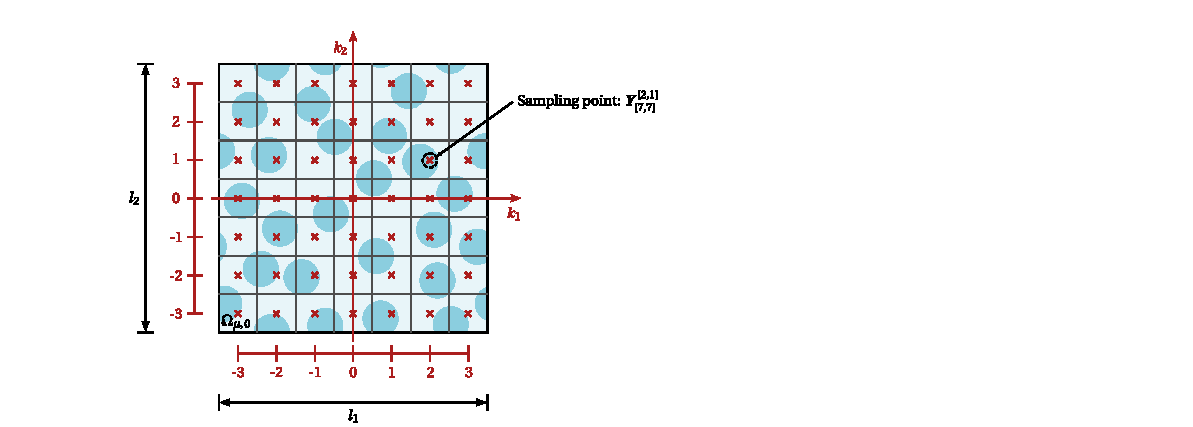
\includegraphics{figures/fft_discretization}
  \caption{Discretization of the periodic cell \(\Omega_{\mu,0}\) with \(\bm n_v = [7,7]\) to be used in the FFT-based homogenization procedure.}
\label{fig:fft_discretization}
\end{figure}

As explained below, only grids with an odd number of nodes will be considered.
For the extension to even grids see Appendix~\ref{app:fft}.
The individual nodes are indexed by a parameter \(\bm k\) from a reduced index set
\begin{equation}
\mathbb{Z}_{\bm n_v}^{d}=\left\{\bm{ k} \in \mathbb{Z}^{d}\ |\ \forall i \in [1,d]\cap \mathbb Z \left(-\frac{n_{v,i}}{2}< k_{i}<\frac{n_{v,i}}{2}\right) \right\}\quad \text{with \(d=2\) or 3},
\end{equation}
and it will become clear later that the indices \(\bm  k\) can be naturally identified with the discrete frequencies from \eqref{eq:compatibility_equations}.
Finally, the integration weight \(w=v_{\mu,0} /n_v\) is set equal to the pixel/voxel size, corresponding to each node.

It is convenient to use the {fundamental trigonometric polynomials} defined on the grid \(\mathbb{Z}_{\bm n_v}^{d}\),
\begin{equation}\label{eq:fundamental_trigonometric_polynomials}
\varphi_{\bm n_v}^{\bm k}(\bm{Y})=\frac{1}{n_v} \sum_{\bm{ m} \in \mathbb{Z}_{\bm n_v}^{d}} \omega_{\bm n_v}^{-\bm{ k  m}} \varphi^{\bm  m}(\bm{ Y})\quad \text { for } \bm{ k} \in \mathbb{Z}_{\bm n_v}^{d},
\end{equation}
as the basis functions to approximate the weak form in Equation~\eqref{eq:form_to_be_discretized}.
Here, \(\varphi^{\bm  m}\) stands for the Fourier basis function (Equation~\eqref{eq:fourier_basis_functions})) and \(\omega_{\bm n_v}^{\bm  k \bm m}\) are the complex-valued coefficients of the Discrete Fourier Transform (DFT),
\begin{equation} \label{eq:def_dft_coefficients}
\omega_{\bm n_v}^{\bm  k \bm  m}=\omega_{\bm n_v}^{\bm  m\bm  k}=\varphi^{\bm  k}\left(\bm Y_{\bm n_v}^{\bm  m}\right)=\exp \left(\mathrm{i}\bm Y_{\bm n_v}^{\bm  k}\cdot \bm \zeta (\bm m)\right) \text { for } \bm{ k}, \bm{ m} \in \mathbb{Z}_{\bm n_v}^{d}.
\end{equation}

The solution \(\tilde{\bm\varepsilon}_\mu\) and the test functions \(\bm \xi\) in Equation~\eqref{eq:convolution_projection_operator} will be approximated as a linear combination of the basis functions \(\varphi_{\bm n_v}^{\bm  k}\); the corresponding approximation space of the tensor-valued trigonometric polynomials will be referred to as \(\pazocal{T}_{\bm n_v}\).
These approximations are conforming, i.e., \(\pazocal{T}_{\bm n_v} \subset \pazocal{H}\), as long as the number of nodes \(n_v\) is odd.
This conformity is lost when \(n_v\) is even, resulting in a more elaborate treatment.

The computational convenience of trigonometric polynomials follows from the fact that they can be efficiently manipulated using the Fast Fourier Transform (FFT), because of (i) the involvement of the DFT coefficients \(\omega_{\bm n_v}^{\bm  k\bm  m}\) in Equation~\eqref{eq:fundamental_trigonometric_polynomials} and (ii) the ability to work with quantities defined in the Fourier space, because they incorporate the Fourier basis functions \(\varphi^{\bm m}\).

In what follows, the most important steps needed to discretize the weak form in Equation~\eqref{eq:weak_form_equilibrium_eq} are collected.

As can be seen from the example in Figure~\ref{fig:example_fundamental_polynomial}, in the real space the fundamental trigonometric polynomials are not locally supported, unlike the conventional Finite Element shape functions, however they are still interpolatory and form the partition-of-unity, because they satisfy
\begin{equation} \label{eq:delta_property}
\varphi_{\bm n_v}^{\bm  k}\left(\bm   Y_{\bm n_v}^{\bm  m}\right)=\delta^{\bm  k \bm  m} \text { for } \bm  k, \bm  m \in \mathbb{Z}_{\bm n_v}^{d}, \quad \sum_{\bm  k \in \mathbb{Z}_{\bm n_v}^{2}} \varphi_{\bm n_v}^{\bm  k}(\bm Y)=1 \text { for } \bm Y \in \Omega_{\mu,0},
\end{equation}
where \(\delta^{\bm  k \bm  m}\) is the Kronecker delta.
In the Fourier domain, they are locally supported on \(\mathbb{Z}_{\bm n_v}^{d}\),
\begin{equation} \label{eq:basis_functions_compact_suppport}
\breve{\varphi}_{\bm n_v}^{\bm  k}(\bm{ m})=0\ \text { for } \bm{ k} \in \mathbb{Z}_{\bm n_v}^{d}, \bm  m \in \mathbb{Z}^{d} \backslash \mathbb{Z}_{\bm n_v}^{d},
\end{equation}
because their definition (Equation~\eqref{eq:fundamental_trigonometric_polynomials}) contains only the Fourier basis functions \(\varphi^{\bm  m}\) associated with the frequencies from the grid \(\mathbb{Z}_{\bm n_v}^{d}\).

\begin{figure}
  \centering
  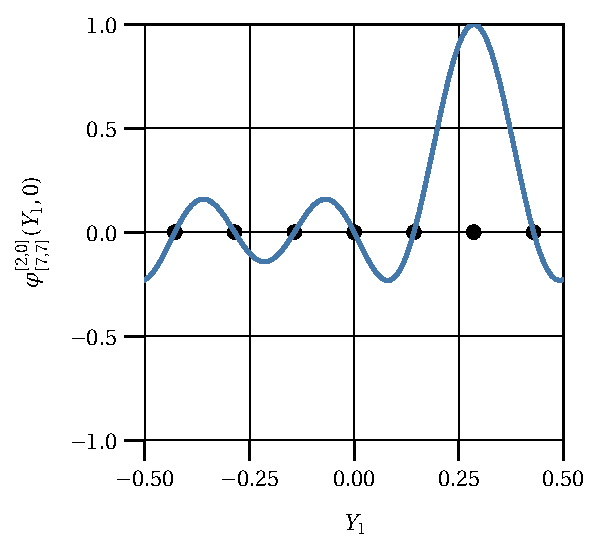
\includegraphics[width=0.55\textwidth]{figures/fundamental_trig_pol}
  \caption{Plot of the fundamental polynomial \(\varphi_{[7,7]}^{[2,0]}(\bm Y)\) for \(-0.5\leq Y_1\leq 0.5\) and \(Y_2=0\). The sampling points are shown as black markers.}
\label{fig:example_fundamental_polynomial}
\end{figure}

As a consequence, every trigonometric polynomial \(\bm\tau \in \pazocal{T}_{\bm n_v}\) admits two equivalent representations on the same grid \(\mathbb{Z}_{\bm n_v}^{d}\) that involve its nodal values \(\bm\tau\left(\bm{Y}_{\bm n_v}^{\bm{ k}}\right)\), and the Fourier coefficients \(\breve{\bm{\tau}}(\bm{ k})\).
Their mutual relation is established by the forward and inverse DFTs,
\begin{gather} \label{eq:forward_fft}
\breve{\bm\tau}(\bm{ k})=\mathcal{DFT}\big (\bm \tau\big )(\bm k)=\frac{1}{n_v} \sum_{\bm  m \in \mathbb{Z}_{\bm n_v}^{d}} \omega_{\bm n_v}^{-\bm  k \bm  m} \bm{\tau}\left(\bm{Y}_{\bm n_v}^{\bm  m}\right)\quad \text { for } \bm{ k} \in \mathbb{Z}_{\bm n_v}^{d},\\
\label{eq:backward_fft}
 \bm{\tau}\left(\bm{Y}_{\bm n_v}^{\bm{ k}}\right)=\mathcal{DFT}^{-1}\big (\breve{\bm \tau}\big )(\bm{Y}_{\bm n_v}^{\bm{ k}})=\sum_{\bm  m \in \mathbb{Z}_{\bm n_v}^{d}} \omega_{\bm n_v}^{\bm  k \bm  m} \breve{\bm{\tau}}(\bm{ m})\quad \text { for } \bm{ k} \in \mathbb{Z}_{\bm n_v}^{d}.
\end{gather}

\subsection{Numerical integration}

The scalar product of two trigonometric polynomials \(\bm\tau \in \pazocal{T}_{\bm n_v}\) and \(\bm{\theta} \in \pazocal{T}_{\bm n_v}\) can be evaluated exactly by the trapezoidal rule,
\begin{equation} \label{eq:trapezoidal_rule}
\int_{\Omega_{\mu,0}} \bm\tau(\bm Y): \bm\theta(\bm Y) \mathrm{d} v=w \sum_{\bm{ k} \in \mathbb{Z}_{\bm n_v}^{d}} \bm{\tau}\left(\bm{Y}_{\bm n_v}^{\bm k}\right): \bm{\theta}\left(\bm{Y}_{\bm n_v}^{\bm{ k}}\right),
\end{equation}
which assigns the same integration weight, equal to the pixel area \(w\), to each grid node.

\subsection{Convolution}

Convolution. of a trigonometric polynomial \(\bm\tau \in \pazocal{T}_{n_v}\) with the projection operator \(\boldsf G\) from \eqref{eq:compatibility_of_test_functions} can be evaluated efficiently at the grid nodes \(\bm Y_{\bm n_v}^{\bm  k}\) by DFT.
Accordingly, from Equation~\eqref{eq:convolution_projection_operator} one finds
\begin{equation}
[\boldsf{G} * \bm{\tau}]\left(\bm{Y}_{\bm n_v}^{\bm  k}\right) = \sum_{\bm  m \in \mathbb{Z}^{d}} \breve{\boldsf{G}}(\bm{ m}):\left[\breve{\bm{\tau}}(\bm{ m}) \varphi^{\bm  m}\left(\bm{Y}_{\bm n_v}^{\bm  k}\right)\right].
\end{equation}
Noting that in the frequency domain the basis functions have compact support (Equation~\eqref{eq:basis_functions_compact_suppport}) and applying the definition for the coefficients of the DFT (Equation~\eqref{eq:def_dft_coefficients}), yields
\begin{equation}
  \sum_{\bm  m \in \mathbb{Z}^{d}} \breve{\boldsf{G}}(\bm{ m}):\left[\breve{\bm{\tau}}(\bm{ m}) \varphi^{\bm  m}\left(\bm{Y}_{\bm n_v}^{\bm  k}\right)\right] = \sum_{\bm  m \in \mathbb{Z}_{\bm n_v}^{d}}  \breve{\boldsf{G}}(\bm{ m}):\left[\breve{\bm\tau}(\bm{ m}) \omega_{\bm n_v}^{\bm  k \bm  m}\right].
\end{equation}
Thus, from the definition of the Discrete Fourier Transform in Equation~\eqref{eq:forward_fft}, the desired result is achieved
\begin{equation}
[\boldsf{G} * \bm{\tau}]\left(\bm{Y}_{\bm n_v}^{\bm  k}\right) = \sum_{\bm  m \in \mathbb{Z}_{\bm n_v}^{d}} \omega_{\bm n_v}^{\bm  k \bm  m} \breve{\boldsf{G}}(\bm{ m}):\left[\frac{1}{n_v} \sum_{\bm  n \in \mathbb{Z}_{\bm n_v}^{d}}
\omega_{\bm n_v}^{-\bm  m \bm  n} \bm{\tau}\left(\bm{Y}_{\bm n_v}^{\bm  n}\right)\right],
\end{equation}
which can be written in a more compact form as
\begin{equation} \label{eq:main_computation_short}
[\boldsf{G} * \bm{\tau}]\left(\bm{Y}_{\bm n_v}^{\bm  k}\right)= \mathcal{DFT}^{-1}\left(\tilde{\boldsf G}:\mathcal{DFT}\left(\bm \tau\right)\right)\left(\bm{Y}_{\bm n_v}^{\bm  k}\right).
\end{equation}

For the non-zero frequency \(\bm k \in \mathbb{Z}_{\bm n_v}^{d} \backslash\{\bm 0\}\), the Fourier transform of the fourth-order projection operator \(\breve{\boldsf G}\) is provided by
\begin{equation} \label{eq:projection_operator_small_strains}
\begin{aligned}
\breve{\boldsf G}_{i j l m}(\boldsymbol{k})=& \frac{1}{2} \frac{\zeta_{i}(\boldsymbol{k}) \delta_{j l} \zeta_{m}(\boldsymbol{k})+\zeta_{i}(\boldsymbol{k}) \delta_{j m} \zeta_{l}(\boldsymbol{k})+\zeta_{j}(\boldsymbol{k}) \delta_{i l} \zeta_{m}(\boldsymbol{k})+\zeta_{j}(\boldsymbol{k}) \delta_{i m} \zeta_{l}(\boldsymbol{k})}{\|\boldsymbol{\zeta}(\boldsymbol{k})\|^{2}} \\
&-\frac{\zeta_{i}(\boldsymbol{k}) \zeta_{j}(\boldsymbol{k}) \zeta_{l}(\boldsymbol{k}) \zeta_{m}(\boldsymbol{k})}{\|\boldsymbol{\zeta}(\boldsymbol{k})\|^{4}},
\end{aligned}
\end{equation}
where \(\zeta_{i}\) are the scaled frequencies and \(\delta_{i j}\) stands for the Kronecker delta.
For \(\boldsymbol{k}=\mathbf{0}\), \(\breve{\boldsf G}_{i j l m}(\mathbf{0})=0\) because of the zero-mean property.

\section{Discretization}

One is now in a position to discretize the weak form of Equation~\eqref{eq:weak_form_equilibrium_eq} with trigonometric polynomials.
Following the standard Galerkin procedure, the unknown field \(\tilde{\bm \varepsilon}_\mu\) and the test field \(\bm \xi\) are approximated in the same way
\begin{align}
\tilde{\bm\varepsilon}_\mu(\bm{Y}) &\approx \sum_{\bm  m \in \mathbb{Z}_{\bm n_v}^{d}} \varphi_{\bm n_v}^{\bm  m}(\bm{Y}) \tilde{\bm \varepsilon}_\mu \left(\bm Y_{\bm n_v}^{\bm  m}\right), \\
\bm \xi(\bm{Y}) &\approx \sum_{\bm  m \in \mathbb{Z}_{\bm n_v}^{d}} \varphi_{\bm n_v}^{\bm m}(\bm{Y}) \bm \xi\left(\bm{Y}_{\bm n_v}^{\bm  m}\right).
\end{align}

The nodal strains, \(\tilde{\bm\varepsilon}_\mu\left(\bm Y_{\bm n_v}^{\bm  m}\right)\) for \(\bm m\in \mathbb Z^d_{\bm n_v}\), and the nodal values of test fields, \(\bm \xi\left(\bm Y_{\bm n_v}^{\bm  m}\right)\) for \(\bm m\in \mathbb Z^d_{\bm n_v}\), are respectively located in the corresponding finite-dimensional spaces \(\mathbb{E}_{\bm n_v} \subset \mathbb{T}_{\bm n_v}\).
The (constrained) space \(\mathbb{E}_{\bm n_v}\) thus collects the nodal values of compatible trigonometric polynomials from \(\pazocal{T}_{\bm n_v} \cap \pazocal{E}\), whereas (unconstrained) \(\mathbb{T}_{\bm n_v}\) collects nodal values of all trigonometric polynomials from \(\pazocal{T}_{\bm n_v}\).

Introducing these expansions into Equation~\eqref{eq:form_to_be_discretized} yields
\begin{equation}
\int_{\Omega_{\mu,0}}\Big(\sum_{\bm  m \in \mathbb{Z}_{\bm n_v}^{d}} \varphi_{\bm n_v}^{\bm  m}(\bm{Y}) \bm\xi\left(\bm{Y}_{\bm n_v}^{\bm  m}\right)  \Big ):[\boldsf{G} * \bm{\sigma}_\mu]\Big(\bm{Y}, \bm{\varepsilon}(\bm X)+\sum_{\bm  m \in \mathbb{Z}_{\bm n_v}^{d}} \varphi_{\bm n_v}^{\bm  m}(\bm{Y}) \tilde{\bm \varepsilon}_\mu \left(\bm Y_{\bm n_v}^{\bm  m}\right) \Big) \mathrm{d} v=0,
\end{equation}
to be satisfied for arbitrary \(\bm\xi\left(\bm{Y}_{\bm n_v}^{\bm  m}\right)\) from \(\mathbb T_{n_v}\), \(\bm m \in \mathbb Z^d_{\bm n_v}\).
Application of the trapezoidal quadrature rule (Equation~\eqref{eq:trapezoidal_rule}) provides
\begin{equation}
w \sum_{\bm  k \in \mathbb{Z}_{\bm n_v}^{d}}\Big(\sum_{\bm  m \in \mathbb{Z}_{\bm n_v}^{d}} \varphi_{\bm n_v}^{\bm  m}(\bm Y_{\bm n_v}^{\bm  k}) \bm\xi\left(\bm{Y}_{\bm n_v}^{\bm  m}\right)\Big):[\boldsf G * \bm{\sigma}_\mu]\Big(\bm Y_{\bm n_v}^{\bm  k}, \bm \varepsilon(\bm X)+\sum_{\bm  m \in \mathbb{Z}_{\bm n_v}^{d}} \varphi_{\bm n_v}^{\bm  m}\left(\bm Y_{\bm n_v}^{\bm  k}\right) \tilde{\bm \varepsilon}_\mu \left(\bm Y_{\bm n_v}^{\bm  m}\right)\Big) \approx 0,
\end{equation}
note that this step introduces an approximation error because the constitutive relation \(\bm{\sigma}_\mu\) does not necessarily map trigonometric polynomials to trigonometric polynomials.
By exploring the Kronecker delta property of the basis functions (Equation~\eqref{eq:delta_property}), the previous relation further simplifies to
\begin{equation} \label{eq:final_variational_form}
\sum_{\bm  k \in \mathbb{Z}_{\bm n_v}^{d}} \bm\xi\left(\bm{Y}_{\bm n_v}^{\bm  k}\right):[\boldsf G * \bm\sigma_\mu]\Big(\bm Y_{\bm n_v}^{\bm k}, \bm \varepsilon(\bm X)+\tilde{\bm \varepsilon}_\mu \left(\bm Y_{\bm n_v}^{\bm  k}\right)\Big)=0.
\end{equation}

Because the test strains \(\bm \xi(\bm Y_{\bm n_v}^{\bm k})\), for \(\bm k\in \mathbb Z^{d}_{\bm n_v}\), are arbitrary, one finally obtains from \eqref{eq:final_variational_form} that the nodal strain values, \(\tilde{\bm\varepsilon}_\mu(\bm Y_{\bm n_v}^{\bm k}) \in \mathbb{E}_{\bm n_v}\), for \(\bm k\in \mathbb Z^{d}_{\bm n_v}\), follow from the system of non-linear nodal equilibrium conditions,
\begin{equation} \label{eq:final_form_sum}
[\boldsf G * \bm\sigma_\mu]\Big(\bm Y_{\bm n_v}^{\bm k}, \bm \varepsilon(\bm X)+\tilde{\bm \varepsilon}_\mu \left(\bm Y_{\bm n_v}^{\bm  k}\right)\Big)=\bm 0\quad \text{for \( \bm k \in \mathbb Z^d_{\bm n_v}\)},
\end{equation}
which can be also be written as
\begin{equation} \label{eq:non_linear_equilibrium_equations}
\mathcal{DFT}^{-1}\left(\tilde{\boldsf G}:\mathcal{DFT}\left(\bm \sigma_\mu\right)\right)\left(\bm{Y}_{\bm n_v}^{\bm  k}, \bm \varepsilon(\bm X)+\tilde{\bm \varepsilon}_\mu \left(\bm Y_{\bm n_v}^{\bm  k}\right)\right)= \bm 0\quad \text{for \(\bm k \in \mathbb Z^d_{\bm n_v}\)}.
\end{equation}
where the non-linearity originates solely from the constitutive relation, because the projection operator \(\boldsf G\) is independent of \(\tilde{\bm\varepsilon}_\mu\).

Therefore, apart from enforcing the strain compatibility, the symmetric matrix \(\boldsf G\) also enforces the nodal equilibrium conditions.
Also notice that, in analogy to Section~\ref{sec:compatibility}, the constraint \(\tilde{\bm\varepsilon}_\mu(\bm Y_{\bm n_v}^{\bm k}) \in \mathbb{E}_{\bm n_v}\), for \(\bm k\in \mathbb Z^{d}_{\bm n_v}\), still needs to be accounted for.

\section{Linearization} \label{sec:linearization}

The conventional Newton scheme is used to find the solution to the system \eqref{eq:non_linear_equilibrium_equations} iteratively. For this purpose, we express the nodal unknowns in the \((i+1)\)-th iteration as
\begin{equation}
\tilde{\bm\varepsilon}_{\mu}^{(i+1)}\left(\bm{Y}_{\bm n_v}^{\bm  k}\right) =\tilde{\bm\varepsilon}_{\mu}^{(i)}\left(\bm{Y}_{\bm n_v}^{\bm  k}\right)+\delta \tilde{\bm\varepsilon}_{\mu}\left(\bm{Y}_{\bm n_v}^{\bm  k}\right)\quad \text{for \(\bm k \in \mathbb Z^d_{\bm n_v}\)}.
\end{equation}
Equation~\eqref{eq:non_linear_equilibrium_equations} is then linearized around \(\tilde{\bm\varepsilon}_\mu^{(i)}\), with \(\tilde{\bm\varepsilon}_\mu^{(0)}\left(\bm{Y}_{\bm n_v}^{\bm  k}\right) \in \mathbb{E}_{\bm n_v}\), for \(\bm k\in \mathbb Z^{d}_{\bm n_v}\).
As a result, one obtains the linear system for the nodal strain increment \(\delta \tilde{\bm\varepsilon}_\mu\left(\bm{Y}_{\bm n_v}^{\bm  k}\right) \in \mathbb{E}_{\bm n_v}\), for \(\bm k\in \mathbb Z^{d}_{\bm n_v}\),
\begin{multline} \label{eq:linearized_equilibrium_equations}
[\boldsf G * \boldsf D^{(i)}]\left(\bm{Y}_{\bm n_v}^{\bm  k}, \bm \varepsilon(\bm X)+\tilde{\bm \varepsilon}_\mu \left(\bm Y_{\bm n_v}^{\bm  k}\right)\right)\delta \tilde{\bm\varepsilon}_{\mu}^{(i+1)}\left(\bm{Y}_{\bm n_v}^{\bm  k}\right)\\ = -[\boldsf G * \bm\sigma_\mu]\left(\bm{Y}_{\bm n_v}^{\bm  k}, \bm \varepsilon(\bm X)+\tilde{\bm \varepsilon}_\mu \left(\bm Y_{\bm n_v}^{\bm  k}\right)\right)\quad \text{for \(\bm k \in \mathbb Z^d_{\bm n_v}\)},
\end{multline}
where the local tangent matrix \(\boldsf D^{(i)}\) is given by
\begin{equation}
\boldsf D^{(i)}\left(\bm{Y}_{\bm n_v}^{\bm  k}, \bm \varepsilon(\bm X)+\tilde{\bm \varepsilon}_\mu \left(\bm Y_{\bm n_v}^{\bm  k}\right)\right)=\frac{\partial \bm{\sigma}_\mu}{\partial \bm \varepsilon_\mu}\left(\bm{Y}_{\bm n_v}^{\bm  k}, \bm \varepsilon(\bm X)+\tilde{\bm \varepsilon}_\mu \left(\bm Y_{\bm n_v}^{\bm  k}\right)\right) \text { for } \bm  k \in \mathbb{Z}_{\bm n_v}^{d}.
\end{equation}

Three considerations must be taken into account when solving the linearized system (Equation~\eqref{eq:linearized_equilibrium_equations}):
\begin{enumerate}[(i)]
  \item the corresponding system matrix is dense, singular, and very costly to assemble for large grids;
  \item the multiplication with the system matrix is cheap and does not require the matrix assembly, because it involves the multiplication with structurally sparse matrices (recall that the convolution with \(\boldsf G\) can be performed efficiently by FFT (Equation~\eqref{eq:main_computation_short}); and
  \item the solver must enforce the compatibility constraint \(\tilde{\bm \varepsilon}_\mu^{(i+1)}\left(\bm{Y}_{\bm n_v}^{\bm  k}\right) \in \mathbb{E}_{\bm n_v}\), for \(\bm k\in \mathbb Z^{d}_{\bm n_v}\).
\end{enumerate}

All these aspects invite the application of (projected) iterative solvers involving only matrix-vector products, such as specific-purpose solvers \citep{moulinec_comparison_2014}, or selected general-purpose iterative algorithms for symmetric positive systems \citep{mishra_comparative_2016}, because the operator \(\boldsf G\) enforces the compatibility and equilibrium conditions simultaneously.
Specifically, we will use the conventional Conjugate Gradient algorithm \citep{hestenes_methods_1952}, which enforces the compatibility constraint at every iteration and outperforms alternative solvers in terms of convergence rate, as demonstrated in \cite{mishra_comparative_2016}.

\section{Algorithm}

To summarize, the incremental-iterative Newton-Conjugate Gradient solver is outlined as a pseudo-algorithm in Box~\ref{box:alg_newton_cg}.
For later reference, it is emphasized that the algorithm implements two termination criteria for the Newton and the Conjugate Gradient solvers that involve the two tolerances \(\eta^{\mathrm{NW}}\) and \(\eta^{\mathrm{CG}}\), respectively.
Finally, note that the same procedure applies to history- and rate-dependent material laws, once the time-incremental stress-strain laws and consistent constitutive tangents are adopted, replacing \(\bm\sigma_\mu^{(i)}\) and \(\boldsf D^{(i)}\) in Equation~\eqref{eq:linearized_equilibrium_equations}.

\begin{framedbox}[htb]
\caption{Pseudo-code for the Newton-CG algorithm solving the equilibrium problem for non-linear behavior.}
\label{box:alg_newton_cg}
\begin{center}
\begin{minipage}{0.9\textwidth}
\begin{enumerate}[(i)]
\item Set the initial conditions: \(t=t_0\)
\item Set strain fluctuations to zero: \(\tilde{\bm \varepsilon}_\mu^{(0)}(\bm Y^{\bm k}_{\bm n_v})=\bm{0}\) for \(\bm  k \in \mathbb{Z}_{\bm n_v}^{d}\)
\item Initialize other history variables (material dependent)
\item Enter increment loop
\begin{enumerate}[(1)]
  \item Set Newton counter to zero: \(i=0\)
  \item Initialize, indicating no convergence yet: \(\delta \tilde{\bm\varepsilon}_\mu(\bm Y^{\bm k}_{\bm n_v})={\bm \infty}\) for \(\bm  k \in \mathbb{Z}_{\bm n_v}^{d}\)
  \item Enter Newton loop
  \begin{enumerate}[(a)]
    \item Compute the constitutive response (material dependent): \[\bm{\sigma}_\mu^{(i)}(\bm Y^{\bm k}_{\bm n_v})={\bm{\sigma}_\mu}\left(\bm{Y}_{\bm n_v}^{\bm  k}, \bm \varepsilon(\bm X)+\tilde{\bm \varepsilon}_\mu \left(\bm Y_{\bm n_v}^{\bm  k}\right)\right)\quad\text{for \(\bm  k \in \mathbb{Z}_{\bm n_v}^{d}\)}\]
    \item Compute the consistent tangent (material dependent):
    \[{\boldsf D}^{(i)}(\bm Y^{\bm k}_{\bm n_v})=\frac{\partial \bm{\sigma}_\mu}{\partial \bm\varepsilon_\mu}\left(\bm{Y}_{\bm n_v}^{\bm  k}, \bm \varepsilon(\bm X)+\tilde{\bm \varepsilon}_\mu \left(\bm Y_{\bm n_v}^{\bm  k}\right)\right)\quad\text{for \(\bm  k \in \mathbb{Z}_{\bm n_v}^{d}\)}\]
    \item Use the standard Conjugate Gradient method to solve
    \[
[\boldsf G * \boldsf D^{(i)}]\left(\bm{Y}_{\bm n_v}^{\bm  k}\right)\delta \tilde{\bm\varepsilon}_{\mu}\left(\bm{Y}_{\bm n_v}^{\bm  k}\right) = -[\boldsf G * \bm\sigma_\mu^{(i)}]\left(\bm{Y}_{\bm n_v}^{\bm  k}\right)\quad \text{for \(\bm k \in \mathbb Z^d_{\bm n_v}\)}
\]
until the desired accuracy \(\eta^{CG}\) is reached.
  \item Update the strain: \({\tilde{\bm\varepsilon}_\mu}^{(i+1)}\left(\bm{Y}_{\bm n_v}^{\bm  k}\right)={\tilde{\bm\varepsilon}_\mu}^{(i)}\left(\bm{Y}_{\bm n_v}^{\bm  k}\right)+\delta {\tilde{\bm\varepsilon}_\mu}\left(\bm{Y}_{\bm n_v}^{\bm  k}\right)\)
  \item If the desired accuracy \(\eta^{\mathrm{NW}}\) has not been reached, update \(i=i+1\) and go to step (a).
  \end{enumerate}
\item Set the "intial guess" for the next increment: \({\tilde{\bm\varepsilon}_\mu}^{(t+\Delta t)}\left(\bm{Y}_{\bm n_v}^{\bm  k}\right)={\tilde{\bm\varepsilon}_\mu}^{(i)}\left(\bm{Y}_{\bm n_v}^{\bm  k}\right)\)
\item Update other history variables (material dependent)
\item If \(t\leq T_0\), proceed to next increment \(t=t+\Delta t\) and go to step (1).
\end{enumerate}
\end{enumerate}
\end{minipage}
\end{center}
\end{framedbox}


\section{Extension to finite strain}

This section presents the adaptations needed to extend the scheme introduced above to finite strains.

\subsection{Problem statement}

The goal is again to solve for the static mechanical equilibrium in the periodic cell for a given applied overall deformation.
The balance of linear momentum, pulled-back to the (undeformed) reference configuration, reads
\begin{equation} \label{eq:equilibrium_equation_finite_strain}
\operatorname{div}_0 \bm{P}_\mu=\bm{0}
\end{equation}
involving the divergence with respect to the reference configuration of the transposed first Piola-Kirchhoff stress tensor \(\bm{P}_\mu\).
The stress \(\bm{P}_\mu\) depends non-linearly on the deformation gradient \(\bm{F}_\mu\)
\begin{equation} \label{eq:constitutive_law_finite_strains}
\bm{P}_\mu=\bm{P}_\mu(\bm{F}_\mu).
\end{equation}

\subsection{Weak form}

The integral form is obtained by multiplying \eqref{eq:equilibrium_equation_finite_strain} with test functions \(\delta \bm Y\) and integrating over the reference domain \(\Omega_{\mu,0}\)
\begin{equation}
\int_{\Omega_{\mu,0}} \delta \bm Y \cdot\left(\operatorname{div}_0 \bm{P}_\mu\right) \mathrm{d} v=0,
\end{equation}
which must hold for all periodic \(\delta \bm Y\).
Subsequently, integration by parts is applied in conjunction with Gauss' divergence theorem.
The boundary term that arises vanishes because of periodicity.
The result reads
\begin{equation} \label{eq:weak_form_displacements}
\int_{\Omega_{\mu,0}}\bm{P}_\mu:\left(\operatorname{div}_0 \left(\delta \bm Y\right)\right) \mathrm{d} v=0,
\end{equation}
where \(:\) denotes a double tensor contraction.
To make use of the FFT-based methods, the weak form of Equation~\eqref{eq:weak_form_displacements} is accordingly reformulated using the deformation gradient \(\bm F_\mu\) as
\begin{equation} \label{eq:weak_form_finite_strain}
\int_{\Omega_{\mu,0}}  \bm{P}_\mu:\delta\bm{F}_\mu \mathrm{~d} v=0,
\end{equation}
in which the test functions \(\delta \bm{F}_\mu\) are periodic and compatible.
Note that compatibility is guaranteed when \(\delta \bm{F}_\mu\) is the gradient of a virtual position vector, as in Finite Elements, but now must be enforced as a constraint in conjunction with Equation~\eqref{eq:weak_form_finite_strain}.

\subsection{Projection to a compatible solution space}

As in the case of small strains, the compatibility of the test functions \(\delta \bm{F}_\mu\) is imposed employing a projection operator \(\boldsf{G}\) (different from the previous one).
It maps an arbitrary field \(\bar{\bm A}\) to its compatible part \(\bm A\) through
\begin{equation} \label{eq:projection_finite_strains}
\boldsf{G} * \overline{\bm{A}}=\bm{A},
\end{equation}
wherein \(*\) is the convolution operator.
The convolution can be evaluated in Fourier space as a simple, local, double tensor contraction.
Furthermore, \(\boldsf{G}\) has a simple closed-form expression in Fourier space,
\begin{equation} \label{eq:def_projection_finite_strains}
\breve{\boldsf G}_{i j l m}\left(\bm{k}\right)=\begin{cases}
0 & \text { for } \bm k=\bm{0} \\[5pt]
\displaystyle{\frac{\delta_{i m} \zeta_{j}\left(\bm{k}\right) \zeta_{l}\left(\bm{k}\right)}{\|\bm{\zeta}\|^{2}} } & \text { otherwise }
\end{cases},
\end{equation}
wherein \(\bm{k}\) is the (spatial) frequency vector and \(\zeta_{i}\) are the scaled frequencies that account for the size of the cell through \(\zeta_{i}(\bm k)=2\pi k_{i} / l_{i}\) (with \(l_{i}\) the size of the periodic cell in direction \(i\)).
Its background and interpretation are discussed in Appendix~\ref{app:fft}.

Application of Equation~\ref{eq:projection_finite_strains} to the weak form of Equation~\ref{eq:weak_form_finite_strain} results in
\begin{equation} \label{eq:finite_strain_eq_to_discretize}
\int_{\Omega_{\mu,0}}(\boldsf{G} * \delta \bar{\bm{F}}_\mu): \bm{P}_\mu^{T} \mathrm{d} v=\int_{\Omega_{\mu,0}} \delta \bar{\bm{F}}_\mu:(\boldsf{G} * \bm{P}_\mu) \mathrm{d} v = 0,
\end{equation}
whereby the symmetry of \(\boldsf{G}\) has been used. Equation~\eqref{eq:finite_strain_eq_to_discretize} should now hold for arbitrary, i.e. not necessarily compatible, periodic test functions \(\delta \bar{\bm{F}}_\mu\).
Please note that the deformation gradient \(\bm{F}_\mu\), hidden in the stress \(\bm{P}_\mu\) through Equation~\eqref{eq:constitutive_law_finite_strains}, should still satisfy the compatibility constraint.

\subsection{Discretization}

Adopting a Galerkin scheme, the unknown field \(\bm{F}_\mu\) and the test functions \(\delta \bar{\bm{F}}_\mu\) are discretized in the same way.
Like in Finite Elements, the continuous fields \(\bm{F}_\mu\) and \(\delta \bar{\bm{F}}_\mu\) are approximated by a finite number of \(n\) nodal values that are multiplied with shape functions associated with each node, i.e.
\begin{gather}
\bm{F}_\mu(\bm Y)  \approx \sum_{\bm m\in\mathbb{Z}^d_{\bm n_v} } \varphi_{\bm n_v}^{\bm m}(\bm Y) \bm{F}_\mu (\bm Y^{\bm m}_{\bm n_v}), \\
\delta \bar{\bm{F}}_\mu(\bm Y) \approx \sum_{\bm m\in\mathbb{Z}^d_{\bm n_v} } \varphi_{\bm n_v}^{\bm m}(\bm Y) \bar{\bm{F}}_\mu (\bm Y^{\bm m}_{\bm n_v}).
\end{gather}
Just as before, the fundamental trigonometric polynomials are used as shape functions.

The discretization is applied to the weak form (Equation~\eqref{eq:finite_strain_eq_to_discretize}) which therefore becomes
\begin{equation} \label{eq:finite_strains_final_variational}
\int_{\Omega_{\mu,0}} \Big(\sum_{\bm m\in\mathbb{Z}^d_{\bm n_v} } \varphi_{\bm n_v}^{\bm m}(\bm Y) \bar{\bm{F}}_\mu (\bm Y^{\bm m}_{\bm n_v})\Big):[\boldsf{G} * \bm{P}_\mu]\Big(\bm Y^{\bm k}_{n_v}, \sum_{\bm m\in\mathbb{Z}^d_{\bm n_v} } \varphi_{\bm n_v}^{\bm m}(\bm Y) \bm{F}_\mu (\bm Y^{\bm m}_{\bm n_v})\Big) \mathrm{d} v=0.
\end{equation}

\subsection{Quadrature}

The integration is again performed using the trapezoidal rule, which applied to Equation~\eqref{eq:finite_strains_final_variational} yields
\begin{equation}
w\sum_{\bm k\in\mathbb{Z}^d_{n_v}} \left(\left(\sum_{\bm m\in\mathbb{Z}^d_{n_v} } \varphi_{\bm n_v}^{\bm m}(\bm Y^{\bm k}_{n_v}) \bar{\bm{F}}_\mu (\bm Y^{\bm m}_{\bm n_v})\right):[\boldsf{G} * \bm{P}_\mu]\left(\bm Y^{\bm k}_{n_v},\sum_{\bm m\in\mathbb{Z}^d_{n_v} } \varphi_{\bm n_v}^{\bm m}(\bm Y^{\bm k}_{n_v}) \bm{F}_\mu (\bm Y^{\bm m}_{\bm n_v})\right)\right)\approx 0.
\end{equation}
The fact that the shape functions can be expressed in terms of the discrete Fourier coefficients is now exploited; and the delta property of the shape functions (Equation~\eqref{eq:delta_property}), writing
\begin{equation} \label{eq:final_form_sum_finite_strain}
\sum_{\bm  k \in \mathbb{Z}_{\bm n_v}^{d}} \bar{\bm{F}}_\mu (\bm Y^{\bm k}_{\bm n_v}):[\boldsf G * \bm P_\mu]\Big(\bm Y_{\bm n_v}^{\bm k}, \bm{F}_\mu (\bm Y^{\bm k}_{\bm n_v})\Big)=0.
\end{equation}

Because the test functions, \(\bar{\bm F}_\mu(\bm Y_{\bm n_v}^{\bm k})\), for \(\bm k\in \mathbb Z^{d}_{\bm n_v}\), are arbitrary, one finally obtains from \eqref{eq:final_form_sum_finite_strain} that the nodal strain values, \({\bm F}_\mu(\bm Y_{\bm n_v}^{\bm k})\), for \(\bm k\in \mathbb Z^{d}_{\bm n_v}\), follow from the system of non-linear nodal equilibrium conditions,
\begin{equation} \label{eq:final_form_sum}
[\boldsf G * \bm P_\mu]\Big(\bm Y_{\bm n_v}^{\bm k}, \bm F_\mu\left(\bm Y_{\bm n_v}^{\bm  k}\right)\Big)=\bm 0\quad \text{for \( \bm k \in \mathbb Z^d_{\bm n_v}\)},
\end{equation}
which can be also be written as
\begin{equation}\label{eq:finite_strain_final_non_lin_eq}
\mathcal{DFT}^{-1}\left(\tilde{\boldsf G}:\mathcal{DFT}\left(\bm P_\mu\right)\right)\left(\bm{Y}_{\bm n_v}^{\bm  k}, \bm F_\mu\left(\bm Y_{\bm n_v}^{\bm  k}\right)\right)= \bm 0\quad \text{for \(\bm k \in \mathbb Z^d_{\bm n_v}\)}.
\end{equation}
where the non-linearity originates solely from the constitutive relation, because the projection operator \(\boldsf G\) is independent of \(\bm F_\mu\).

Therefore, apart from enforcing the strain compatibility, the symmetric matrix \(\boldsf G\) also enforces the nodal equilibrium conditions.
Also notice, that once more, the constraint regarding the compatibility of \(\bm F_\mu\), still needs to be accounted for.

The weak form in Equation~\eqref{eq:finite_strain_final_non_lin_eq} is a non-linear equation, as the material model involves a non-linear relation between the first Piola-Kirchhoff stress and the deformation gradient.
Newton iterations are employed to solve the nodal equilibrium equations~\eqref{eq:finite_strain_final_non_lin_eq}.
To this end the nodal unknowns at iteration \(i+1\) are expressed as
\begin{equation} \label{eq:linearization_finite_strain}
{\bm{F}_\mu}^{(i+1)}\left(\bm Y_{\bm n_v}^{\bm  k}\right)={\bm{F}_\mu}^{(i)}\left(\bm Y_{\bm n_v}^{\bm  k}\right)+\delta {\bm{F}_\mu}\left(\bm Y_{\bm n_v}^{\bm  k}\right)\quad \text{for \(\bm k\in \mathbb Z^d_{\bm n_v}\)},
\end{equation}
where \({\bm{F}_\mu}^{(i)}\) are the last known iterative values of the deformation gradients and \(\delta {\bm{F}_\mu}\) are their iterative updates.
Note that \(\delta\) is now used to indicate a small variation.
The stresses are linearized around \({\bm{F}_\mu}^{(i)}\).
In a material point this corresponds to
\begin{equation} \label{eq:newton_increment}
\delta \bm{P}_\mu=\boldsf{A}^{(i)}: \delta \bm{F}_\mu.
\end{equation}

Combined with the discretized weak form in Equation~\eqref{eq:final_form_sum}, the iterative update \(\delta {\bm{F}_\mu}\) is found by solving the following linearized system
\begin{equation} \label{eq:linear_system_finite_strain}
[\boldsf{G}* \boldsf A^{(i)}] \left(\bm Y_{\bm n_v}^{\bm  k}, \bm F_\mu^{(i)}\left(\bm Y_{\bm n_v}^{\bm  k}\right)\right):\delta {\bm{F}_\mu}\left(\bm Y_{\bm n_v}^{\bm  k}\right)=-[\boldsf{G}* \bm{P}_\mu]\left(\bm Y_{\bm n_v}^{\bm  k}, \bm F_\mu^{(i)}\left(\bm Y_{\bm n_v}^{\bm  k}\right)\right)\quad\text{for \(\bm k\in \mathbb Z^d_{\bm n_v}\)}.
\end{equation}

Note that the compatibility of the deformation gradient field still needs to be enforced.
This is done by solving the linear system of Equation~\eqref{eq:linear_system_finite_strain} using an iterative solver which delivers a compatible solution in each iteration.
To satisfy compatibility during the entire iterative process, projection-based iterative methods such as e.g. the conjugate gradient (CG) method and the generalized minimal residual method (GMRES), Chebyshev iterations, or Richardson iterations (used in the original Moulinec-Suquet algorithm \citep{moulinec_fast_1994, moulinec_fft-based_1995} can be used.
Alternatively, compatibility is satisfied only at convergence for some of the accelerated methods, such as the ones based on polarization.

\subsection{Implementation}

The numerical algorithm requires the solution of Equation \eqref{eq:finite_strain_final_non_lin_eq} in an incremental-iterative fashion.
Each increment thereby consists of Newton iterations updating the nodal deformation gradients \(\bm{F}_\mu^{(i+1)}(\bm Y^{\bm k}_{\bm n_v})\), for \(\bm k\in \mathbb Z^d_{\bm n_v}\) using Equations \eqref{eq:linearization_finite_strain}-\eqref{eq:linear_system_finite_strain} until equilibrium is satisfied up to an accuracy \(\eta^{\mathrm{NW}}\), by employing the linearized constitutive response.
The linear system in Equation~\eqref{eq:linear_system_finite_strain} is solved up to an accuracy \(\eta^{\text {CG }}\) using the conjugate gradient iterative solver.
\paragraph{Boundary conditions}

With the periodic micro-fluctuations of \(\bm{F}_\mu\) following from equilibrium and compatibility, only the macroscopic deformation or stress needs to be prescribed.
Here only a fully prescribed macroscopic deformation gradient is considered \(\bar{\bm{F}}_\mu\), as this is the easiest and the most efficient choice.

The starting point is an equilibrium state given by \({\bm{F}}_\mu^{(0)}\), to which  a macroscopic deformation gradient \(\bar{\bm{F}}_\mu\) is applied.
More specifically, we apply the difference of \(\bm{\bm{F}}\) and to the mean of \({\bm{F}}_\mu^{(0)}\)
\begin{equation}
\Delta \bar{\bm{F}}_\mu\left(\bm Y_{\bm n_v}^{\bm  k}\right)=\bar{\boldsymbol{F}}_\mu\left(\bm Y_{\bm n_v}^{\bm  k}\right)-\int_{\Omega_{\mu,0}} {\bm{F}}_\mu^{(0)}\left(\bm Y_{\bm n_v}^{\bm  k}\right) \mathrm{d} v\quad \text{for \(\bm k \in \mathbb Z^d_{\bm n_v}\)}.
\end{equation}
For the first Newton iteration, equilibrium reads
\begin{equation} \label{eq:first_equilibrium}
[\boldsf{G}* \bm {P}_\mu]\left(\bm Y_{\bm n_v}^{\bm  k},\bm{F}_\mu^{(0)}\left(\bm Y_{\bm n_v}^{\bm  k}\right)+\Delta \bar{\boldsymbol{F}}_\mu\left(\bm Y_{\bm n_v}^{\bm  k}\right)+\delta {\boldsymbol{F}}_\mu\left(\bm Y_{\bm n_v}^{\bm  k}\right)\right)=\bm{0}\quad \text{for \(\bm k \in \mathbb Z^d_{\bm n_v}\)}.
\end{equation}
Linearization of \eqref{eq:first_equilibrium} results in
\begin{multline}\label{eq:first_equilibrium_lin}
[\boldsf{G}* \boldsf{A}^{(0)}]\left(\bm Y_{\bm n_v}^{\bm  k}, \bm F_\mu^{(0)}\left(\bm Y_{\bm n_v}^{\bm  k}\right)\right): \delta \bm{F}_\mu\left(\bm Y_{\bm n_v}^{\bm  k}\right)=\\-[\boldsf{G}* \boldsf{A}^{(0)}]\left(\bm Y_{\bm n_v}^{\bm  k}, \bm F_\mu^{(0)}\left(\bm Y_{\bm n_v}^{\bm  k}\right)\right): \Delta \bar{\bm{F}}\left(\bm Y_{\bm n_v}^{\bm  k}\right)\quad \text{for \(\bm k \in \mathbb Z^d_{\bm n_v}\)},
\end{multline}
where \(\boldsf{A}^{(0)}\) is the constitutive tangent about \({\bm{F}}_\mu^{(0)}\).
Note that use has been made of the fact that \({\bm{F}}_\mu^{(0)}\) is in equilibrium, i.e. that \([\boldsf G * \bm P_\mu]\left(\bm Y_{\bm n_v}^{\bm  k}, {\bm{F}}_\mu^{(0)}\right)={\bm{0}}\).
After solving the system in Equation~\eqref{eq:first_equilibrium_lin} one sets
\begin{equation}
{\bm{F}}_\mu^{(1)}\left(\bm Y_{\bm n_v}^{\bm  k}\right)={\bm{F}}_\mu^{(0)}\left(\bm Y_{\bm n_v}^{\bm  k}\right)+\Delta \bar{\bm{F}}_\mu\left(\bm Y_{\bm n_v}^{\bm  k}\right)+\delta {\bm{F}}_\mu\left(\bm Y_{\bm n_v}^{\bm  k}\right)\quad \text{for \(\bm k \in \mathbb Z^d_{\bm n_v}\)},
\end{equation}
and proceed normally.
It is thereby important to point out that the definition of \(\boldsf{G}\) ensures that the mean
\begin{equation}
\int_{\Omega_{\mu,0}} \delta {\bm {F}} \mathrm{d} v=\boldsymbol{0}.
\end{equation}
All iterations thus satisfy the prescribed \(\bar{\bm{F}}\) exactly.
The interpretation of Equation~\eqref{eq:first_equilibrium_lin} is that, by solving the linear system, the macroscopic deformation, \(\Delta \bar{\bm{F}}\), is distributed over this microstructure using the tangent \(\boldsf{A}^{(0)}\), which contains the microstructural heterogeneity.
Equation~\eqref{eq:first_equilibrium_lin} therefore has strong similarities with the application of essential (Dirichlet) boundary conditions in the Finite Element Method.
\bigskip

Box~\ref{box:alg_newton_cg_finite_strains} presents the pseudo-code for the Newton-CG scheme used to solve the non-linear equilibrium equations at finite strains.

\begin{framedbox}[htb]
\caption{Pseudo-code for the Newton-CG algorithm solving the equilibrium problem for non-linear behavior at finite strains.}
\label{box:alg_newton_cg_finite_strains}
\begin{center}
\begin{minipage}{0.9\textwidth}
\begin{enumerate}[(i)]
\item Initialize \(\bm F_\mu^{(0)}\left(\bm Y^{(k)}_{\bm n_v}\right) = \bm I\) for \(\bm k \in \mathbb Z^d_{\bm n_v}\) and history variables
\item Enter increment loop
\begin{enumerate}[(1)]
  \item Set Newton counter to zero: \(i=0\)
  \item Enter Newton loop
  \begin{enumerate}[(a)]
    \item Compute the constitutive response (material dependent): \(\bm F_\mu^{(i)} \to \boldsf A^{(i)}, \bm P_\mu^{(i)}\)
    \item According to
    \begin{itemize}
      \item If \(i=0\) then enforce the boundary condition:\\
      Solve
      \begin{multline*}
      [\boldsf{G}* \boldsf{A}^{(0)}]\left(\bm Y_{\bm n_v}^{\bm  k}, \bm F_\mu^{(0)}\left(\bm Y_{\bm n_v}^{\bm  k}\right)\right): \delta \bm{F}_\mu\left(\bm Y_{\bm n_v}^{\bm  k}\right)=\\-[\boldsf{G}* \boldsf{A}^{(0)}]\left(\bm Y_{\bm n_v}^{\bm  k}, \bm F_\mu^{(0)}\left(\bm Y_{\bm n_v}^{\bm  k}\right)\right): \Delta \bar{\bm{F}}\left(\bm Y_{\bm n_v}^{\bm  k}\right)\quad \text{for \(\bm k \in \mathbb Z^d_{\bm n_v}\)},
      \end{multline*}
      \begin{equation*}
      {\bm{F}}_\mu^{(1)}\left(\bm Y_{\bm n_v}^{\bm  k}\right)={\bm{F}}_\mu^{(0)}\left(\bm Y_{\bm n_v}^{\bm  k}\right)+\Delta \bar{\bm{F}}_\mu\left(\bm Y_{\bm n_v}^{\bm  k}\right)+\delta {\bm{F}}_\mu\left(\bm Y_{\bm n_v}^{\bm  k}\right)\quad \text{for \(\bm k \in \mathbb Z^d_{\bm n_v}\)},
      \end{equation*}
      \item else, enforce the equilibrium iteration
      \begin{multline*}
      [\boldsf{G}* \boldsf A^{(i)}] \left(\bm Y_{\bm n_v}^{\bm  k}, \bm F_\mu^{(i)}\left(\bm Y_{\bm n_v}^{\bm  k}\right)\right):\delta {\bm{F}_\mu}\left(\bm Y_{\bm n_v}^{\bm  k}\right)= \\
      -[\boldsf{G}* \bm{P}_\mu^{(i)}]\left(\bm Y_{\bm n_v}^{\bm  k}, \bm F_\mu^{(i)}\left(\bm Y_{\bm n_v}^{\bm  k}\right)\right)\quad\text{for \(\bm k\in \mathbb Z^d_{\bm n_v}\)}.
      \end{multline*}
      \begin{equation*}
      {\bm{F}_\mu}^{(i+1)}\left(\bm Y_{\bm n_v}^{\bm  k}\right)={\bm{F}_\mu}^{(i)}\left(\bm Y_{\bm n_v}^{\bm  k}\right)+\delta {\bm{F}_\mu}\left(\bm Y_{\bm n_v}^{\bm  k}\right)\quad \text{for \(\bm k\in \mathbb Z^d_{\bm n_v}\)},
      \end{equation*}
    \end{itemize}
    \item If the desired accuracy \(\eta^{NW}\) has not been reached, update index \(i=i+1\) and go to (a)
  \end{enumerate}
  \item Store the converged state \(\bm F^{(i+1)}\) and the history variables, set \(\bm F^{(0)}_\mu=\bm F^{(i+1)}_\mu\), and go to (1)
\end{enumerate}
\end{enumerate}
\end{minipage}
\end{center}
\end{framedbox}

\section{Convergence criteria} \label{sec:criteria}

Two different convergence criteria are considered in this work and described in what follows.
They include a criterion for the Conjugate Gradient procedure (interior loop) and a criterion for the Newton-Raphson procedure (exterior loop).
Let \(i\) and \(j\) be the current Newton and Conjugate Gradient iteration steps, respectively.

\paragraph{Criterion I}

Criterion I follows from the most common criterion for the Conjugate Gradient.
Since equilibrium is described by Equation~\eqref{eq:final_form_sum}, repeated here for clarity sake,
\begin{equation}
[\boldsf G * \bm P_\mu]\Big(\bm Y_{\bm n_v}^{\bm k}, \bm F_\mu\left(\bm Y_{\bm n_v}^{\bm  k}\right)\Big)=\bm 0\quad \text{for \( \bm k \in \mathbb Z^d_{\bm n_v}\)},
\end{equation}
the linearized version reads
\begin{equation}
[\boldsf{G}* \boldsf A^{(i)}] \left(\bm Y_{\bm n_v}^{\bm  k}, \bm F_\mu^{(i)}\left(Y_{\bm n_v}^{\bm  k}\right)\right):\delta {\bm{F}_\mu}\left(\bm Y_{\bm n_v}^{\bm  k}\right)=-[\boldsf{G}* \bm{P}_\mu]\left(\bm Y_{\bm n_v}^{\bm  k}, \bm F_\mu^{(i)}\left(Y_{\bm n_v}^{\bm  k}\right)\right)\quad\text{for \(\bm k\in \mathbb Z^d_{\bm n_v}\)}.
\end{equation}
Thus, the Conjugate Gradient will converge only when, for CG iteration \(j\), one verifies
\begin{equation}
\frac{\displaystyle{\left\|[\boldsf{G}* \boldsf{A}^{(i)}]: \delta \bm F_\mu^{(j)}+\boldsf{G}* \bm P_\mu^{(i)}\right\|}}{\displaystyle{\left\|\boldsf{G}* \bm P_\mu^{(i)}\right\|}}<\eta^{\mathrm{CG}},
\end{equation}
using as the reference value \(\boldsf G*\bm P_\mu^{(i)}\), where the arguments where droped for clarity.

Regarding the Newton-Raphson procedure, the tangent stiffness is updated and the same expression is used, now with the converged increment \(\delta \bm F\) from the CG method, such that the scheme has converged only when
\begin{equation}
\frac{\displaystyle{\left\|[\boldsf{G}* \boldsf{A}^{(i+1)}]: \delta \bm F_\mu+\boldsf{G}* \bm P_\mu^{(i)}\right\|}}{\displaystyle{\left\|\boldsf{G}* \bm P_\mu^{(i)}\right\|}}<\eta^{\mathrm{NW}}.
\end{equation}

The application of this criterion to the case of small strains is straightforward, needing only the deformation gradient the first Piola-Kirchhoff stress tensor to be replaced by the small strain tensor and the Cauchy stress tensor, respectively.

\paragraph{Criterion II}

Criterion II uses the consecutive values of the stress tensor to ascertain if each of the methods, Conjugate Gradient and Newton-Raphson, have converged.

For the Conjugate Gradient method it reads
\begin{equation}
\frac{\displaystyle{\left\|\bm P_\mu^{(i,j)}-\bm P_\mu^{(i,j+1)}\right\|}}{\displaystyle{\left\|\bm P_\mu^{(i,j+1)}\right\|}}<\eta^{\mathrm{CG}},
\end{equation}
where the \(\bm P_\mu^{(i,j+1)}\) is computed as
\begin{equation}
  \bm P_\mu^{(i,j+1)} = \bm P_\mu^{(i,j)}+ \boldsf A^{(i)}: \delta \bm F_\mu^{(j)},
\end{equation}
and the double superscript indicates the Cojugate Gradient and the Newton-Raphson iteraion.

For the Newton-Raphson procedure, the consequitve values for the stress in the current and the next iteration are used as follows
\begin{equation}
\frac{\displaystyle{\left\|\bm P_\mu^{(i+1)}-\bm P_\mu^{(i)}\right\|}}{\displaystyle{\left\|\bm P_\mu^{(i+1)}\right\|}}<\eta^{\mathrm{NW}}.
\end{equation}

\newpage\null\thispagestyle{blank}\newpage
